% Dokumentklassen:
% article, report, beamer, book, letter etc.
% https://en.wikibooks.org/wiki/LaTeX/Document_Structure
\documentclass[a4paper]{article}

% Seitenränder Abstand setzen
\usepackage[margin=80pt]{geometry}

% Deutsches Sprachpaket
\usepackage[ngerman]{babel}
% UTF8 Input Encoding
\usepackage[utf8]{inputenc}

% Schriftbild ändern
% https://en.wikibooks.org/wiki/LaTeX/Fonts
\usepackage[scaled]{helvet}
% (Sans) Serifen oder anderes
% \rmdefault: Serifen
% \sfdefault: Sans-Serifen
% \ttdefault: Typewriter
\renewcommand{\familydefault}{\sfdefault}
% Fontencoding (für ä, ö, ü etc.)
\usepackage[T1]{fontenc}

% Gänsefüsschen richtig kompilieren
\usepackage [autostyle]{csquotes}
\MakeOuterQuote{"}

% Hyperlinks farblos
\usepackage[hidelinks]{hyperref}
\hypersetup{colorlinks=false}

% Package für Aufzählungen
\usepackage{enumitem}
% kein Abstand zwischen Aufzählungen
% Sollen doch Abstände vorhanden sein: nach Aufzählung {itemsep=1em}
\setlist{nosep}

% Grafik-Packages, für Figures, Subfigures und PDF als Import
\usepackage{graphicx}
\usepackage{subcaption}
\usepackage{pdfpages}

\title{\textbf{Zusammenfassung PMRE}\\
Project Management \& Requirements Engineering}
\date{\today}
\author{Maurin D. Thalmann}

\begin{document}
	
	\pagenumbering{gobble}
	\maketitle
	
	\newpage
	\pagenumbering{arabic}
	\tableofcontents
	
	\newpage
	
	\section{Project Management}
	
		% TODO evtl. Einleitende Gedanken beifügen
	
		\subsection{Projektarbeit \& -Abwicklung}
		
		\begin{description}
			\item[Systemgestaltung] Ein System um- oder neugestalten, um ein erkanntes Problem (unbefriedigenden Zustand) zu lösen
			\item[Problemlösungsprozess (makro)] Problemlösungsvorgehen anwenden, welches durch Projektorganisation und prozessuelles Vorgehen (Phasenplan) strukturiert wird
			\item[Projektmanagement] Projektleitung dirigiert Problemlösungsprozess nach vorgegebener Art und Weise, um Erfolg des Vorhabens sicherzustellen
			\item[Problemlösungszyklus (mikro)] Projektteam wendet im Laufe der Problemlösung Methoden, Techniken, Werkzeuge an, um ein optimales Zielsystem zu gestalten
		\end{description}
	
				\paragraph{Projekt}
				
				Ein Projekt beinhaltet alle Tätigkeiten, um einen IST-Zustand (Problem) in einen Soll-Zustand (Lösung) zu überführen
				
				\paragraph{Projektabwicklung}
				
				Projektabwicklung legt den Fokus auf die Art und Weise der Abwicklung eines Projekts, um ein vereinbartes Projektziel zu erreichen. 
				Meist wird eine vorgegebene Art und Weise des Vorgehens für die konkrete Abwicklung genutzt (Projektmethode a.k.a. Vorgehensmodell oder Vorgehensmethode).
				
				\paragraph{Unterscheidung Projektmanagement vs. Systemgestaltung}
								
				\begin{description}
					\item[Projektmanagement] Fokus auf das Management des Problemlösungsprozesses, die Planung und Disposition der Ressourcen, die Organisation der Informationsflüsse, der Meinungsbildungs- und Entscheidungsprozesse etc.
					\item[Systemgestaltung] auch System Engineering; Fokus auf die Problemlösung im eigentlichen Sinne, die effektive Um- oder Neugestaltung eines Systems
				\end{description}
			
			\subsubsection{Aufgaben des Projektmanagement}
			
			Projektmanagement als Sammelbegriff für alle planenden, überwachenden, koordinierenden und steuernden Tätigkeiten, welche zur erfolgreichen Durchführung der Systemgestaltung notwendig sind.
			Das Vorgehen zur Erreichung der Lösung steht im Vordergrund (nicht das System an sich).
			Projektmanagement lässt sich in folgende Dimensionen gliedern:
			\vspace{1em}
			\begin{description}
				\item[Funktionale Dimension] Alle Aufgaben der Ingangsetzung, Inganghaltung und dem Abschluss eines Projekts
				\item[Institutionale Dimension] dalle Aufgaben, um formale Organisations- und Entscheidungseinheiten zu schaffen, welche im Projekt etabliert werden (Projektteams, Gremien und Rollen)
				\item[Instrumentale Dimension] Alle Aufgaben der Definition, Einführung und Unterhalt von Methoden und Werkzeugen zur zeitlichen, kapazitiven, qualitativen und kostenbezogenen Planung, Überwachung und Steuerung eines Projekts
				\item[Personelle Dimension] Alle personenbezogenen Komponenten in einem Projekt, Wahl von Mitarbeitenden, Zusammenarbeit, Kommunikation, Konfliktbewältigung etc.
				\item[Psychologische Dimension] Alle personenbezogenen Aspekte eines Projekt, bezogen auf Akzeptanz der Ziele, Vorgehensweisen, Verhaltensmuster, Sinnhaftigkeit des Vorhabens durch Mitarbeiter.
			\end{description}
		
			\subsubsection{Aufgaben der Sytemgestaltung}
			
			Bei Systemgestaltung steht die eigentliche Problemlösung / Lösungsfindung im Vordergrund.
			Somit das eigentliche Problem selbst, gedanklicher Lösungsansatz, Abgrenzung zur Umwelt, Anforderungen, die Lösung im engeren inhaltlichen Sinne, Aspekte des Entwurfs, der Architektur des Aufbaus der Lösung, die detaillierte Ausgestaltung etc.
			
			\newpage
			
			\paragraph{Gesamtheitliche Sicht auf die Projektabwicklung}
			
			Die beiden Makroprozesse des Projektmanagement und der Systemgestaltung ergeben eine gesamtheitliche Sicht auf die Abwicklung von Projekten:
		
			\begin{figure}[!htb]
				\centering
				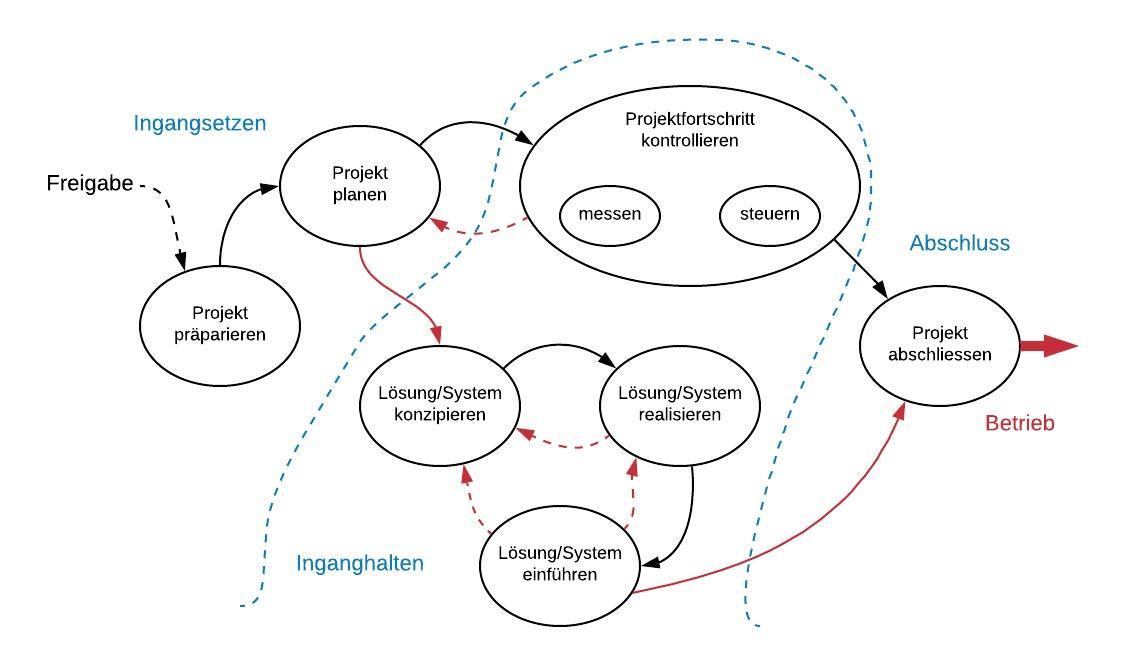
\includegraphics[keepaspectratio, height=6.5cm]{img/pm/project_view.jpeg}
				\caption{Gesamtheitliche Sicht auf Mikroprozesse der Projektabwicklung}
				\label{fig:pm_projectview}
			\end{figure}
		
		
		
				
	\section{Requirements Engineering}
	
		\subsection{title}
		
		
		
		
		
	
	
\end{document}
